% Options for packages loaded elsewhere
\PassOptionsToPackage{unicode}{hyperref}
\PassOptionsToPackage{hyphens}{url}
%
\documentclass[
]{article}
\usepackage{amsmath,amssymb}
\usepackage{lmodern}
\usepackage{ifxetex,ifluatex}
\ifnum 0\ifxetex 1\fi\ifluatex 1\fi=0 % if pdftex
  \usepackage[T1]{fontenc}
  \usepackage[utf8]{inputenc}
  \usepackage{textcomp} % provide euro and other symbols
\else % if luatex or xetex
  \usepackage{unicode-math}
  \defaultfontfeatures{Scale=MatchLowercase}
  \defaultfontfeatures[\rmfamily]{Ligatures=TeX,Scale=1}
\fi
% Use upquote if available, for straight quotes in verbatim environments
\IfFileExists{upquote.sty}{\usepackage{upquote}}{}
\IfFileExists{microtype.sty}{% use microtype if available
  \usepackage[]{microtype}
  \UseMicrotypeSet[protrusion]{basicmath} % disable protrusion for tt fonts
}{}
\makeatletter
\@ifundefined{KOMAClassName}{% if non-KOMA class
  \IfFileExists{parskip.sty}{%
    \usepackage{parskip}
  }{% else
    \setlength{\parindent}{0pt}
    \setlength{\parskip}{6pt plus 2pt minus 1pt}}
}{% if KOMA class
  \KOMAoptions{parskip=half}}
\makeatother
\usepackage{xcolor}
\IfFileExists{xurl.sty}{\usepackage{xurl}}{} % add URL line breaks if available
\IfFileExists{bookmark.sty}{\usepackage{bookmark}}{\usepackage{hyperref}}
\hypersetup{
  pdftitle={Recursive Wordle Solver},
  pdfauthor={Matt Moore},
  hidelinks,
  pdfcreator={LaTeX via pandoc}}
\urlstyle{same} % disable monospaced font for URLs
\usepackage[margin=1in]{geometry}
\usepackage{color}
\usepackage{fancyvrb}
\newcommand{\VerbBar}{|}
\newcommand{\VERB}{\Verb[commandchars=\\\{\}]}
\DefineVerbatimEnvironment{Highlighting}{Verbatim}{commandchars=\\\{\}}
% Add ',fontsize=\small' for more characters per line
\usepackage{framed}
\definecolor{shadecolor}{RGB}{248,248,248}
\newenvironment{Shaded}{\begin{snugshade}}{\end{snugshade}}
\newcommand{\AlertTok}[1]{\textcolor[rgb]{0.94,0.16,0.16}{#1}}
\newcommand{\AnnotationTok}[1]{\textcolor[rgb]{0.56,0.35,0.01}{\textbf{\textit{#1}}}}
\newcommand{\AttributeTok}[1]{\textcolor[rgb]{0.77,0.63,0.00}{#1}}
\newcommand{\BaseNTok}[1]{\textcolor[rgb]{0.00,0.00,0.81}{#1}}
\newcommand{\BuiltInTok}[1]{#1}
\newcommand{\CharTok}[1]{\textcolor[rgb]{0.31,0.60,0.02}{#1}}
\newcommand{\CommentTok}[1]{\textcolor[rgb]{0.56,0.35,0.01}{\textit{#1}}}
\newcommand{\CommentVarTok}[1]{\textcolor[rgb]{0.56,0.35,0.01}{\textbf{\textit{#1}}}}
\newcommand{\ConstantTok}[1]{\textcolor[rgb]{0.00,0.00,0.00}{#1}}
\newcommand{\ControlFlowTok}[1]{\textcolor[rgb]{0.13,0.29,0.53}{\textbf{#1}}}
\newcommand{\DataTypeTok}[1]{\textcolor[rgb]{0.13,0.29,0.53}{#1}}
\newcommand{\DecValTok}[1]{\textcolor[rgb]{0.00,0.00,0.81}{#1}}
\newcommand{\DocumentationTok}[1]{\textcolor[rgb]{0.56,0.35,0.01}{\textbf{\textit{#1}}}}
\newcommand{\ErrorTok}[1]{\textcolor[rgb]{0.64,0.00,0.00}{\textbf{#1}}}
\newcommand{\ExtensionTok}[1]{#1}
\newcommand{\FloatTok}[1]{\textcolor[rgb]{0.00,0.00,0.81}{#1}}
\newcommand{\FunctionTok}[1]{\textcolor[rgb]{0.00,0.00,0.00}{#1}}
\newcommand{\ImportTok}[1]{#1}
\newcommand{\InformationTok}[1]{\textcolor[rgb]{0.56,0.35,0.01}{\textbf{\textit{#1}}}}
\newcommand{\KeywordTok}[1]{\textcolor[rgb]{0.13,0.29,0.53}{\textbf{#1}}}
\newcommand{\NormalTok}[1]{#1}
\newcommand{\OperatorTok}[1]{\textcolor[rgb]{0.81,0.36,0.00}{\textbf{#1}}}
\newcommand{\OtherTok}[1]{\textcolor[rgb]{0.56,0.35,0.01}{#1}}
\newcommand{\PreprocessorTok}[1]{\textcolor[rgb]{0.56,0.35,0.01}{\textit{#1}}}
\newcommand{\RegionMarkerTok}[1]{#1}
\newcommand{\SpecialCharTok}[1]{\textcolor[rgb]{0.00,0.00,0.00}{#1}}
\newcommand{\SpecialStringTok}[1]{\textcolor[rgb]{0.31,0.60,0.02}{#1}}
\newcommand{\StringTok}[1]{\textcolor[rgb]{0.31,0.60,0.02}{#1}}
\newcommand{\VariableTok}[1]{\textcolor[rgb]{0.00,0.00,0.00}{#1}}
\newcommand{\VerbatimStringTok}[1]{\textcolor[rgb]{0.31,0.60,0.02}{#1}}
\newcommand{\WarningTok}[1]{\textcolor[rgb]{0.56,0.35,0.01}{\textbf{\textit{#1}}}}
\usepackage{longtable,booktabs,array}
\usepackage{calc} % for calculating minipage widths
% Correct order of tables after \paragraph or \subparagraph
\usepackage{etoolbox}
\makeatletter
\patchcmd\longtable{\par}{\if@noskipsec\mbox{}\fi\par}{}{}
\makeatother
% Allow footnotes in longtable head/foot
\IfFileExists{footnotehyper.sty}{\usepackage{footnotehyper}}{\usepackage{footnote}}
\makesavenoteenv{longtable}
\usepackage{graphicx}
\makeatletter
\def\maxwidth{\ifdim\Gin@nat@width>\linewidth\linewidth\else\Gin@nat@width\fi}
\def\maxheight{\ifdim\Gin@nat@height>\textheight\textheight\else\Gin@nat@height\fi}
\makeatother
% Scale images if necessary, so that they will not overflow the page
% margins by default, and it is still possible to overwrite the defaults
% using explicit options in \includegraphics[width, height, ...]{}
\setkeys{Gin}{width=\maxwidth,height=\maxheight,keepaspectratio}
% Set default figure placement to htbp
\makeatletter
\def\fps@figure{htbp}
\makeatother
\setlength{\emergencystretch}{3em} % prevent overfull lines
\providecommand{\tightlist}{%
  \setlength{\itemsep}{0pt}\setlength{\parskip}{0pt}}
\setcounter{secnumdepth}{-\maxdimen} % remove section numbering
\ifluatex
  \usepackage{selnolig}  % disable illegal ligatures
\fi

\title{Recursive Wordle Solver}
\usepackage{etoolbox}
\makeatletter
\providecommand{\subtitle}[1]{% add subtitle to \maketitle
  \apptocmd{\@title}{\par {\large #1 \par}}{}{}
}
\makeatother
\subtitle{A reproducible R tutorial}
\author{Matt Moore}
\date{28/01/2022}

\begin{document}
\maketitle

\hypertarget{introduction}{%
\section{Introduction}\label{introduction}}

\hypertarget{why-use-r-to-write-reproducible-reports}{%
\subsection{Why use R to write reproducible
reports?}\label{why-use-r-to-write-reproducible-reports}}

Writing an entire report in R has a significant learning curve, but
comes with many payoffs later down the line. For example, during the
review process, analysis pipelines may change several times. This
requires reported values and figures to be updated everywhere they
appear, potentially leading to errors and discrepancies between the
published results and the actual analysis that took place.

A report written in R can be published along with all the source code
used to generate it, so that anyone can see exactly how you reached your
results and reproduce everything for themselves, using either your data
or their own. Whilst closed-source, proprietary software like MATLAB can
be powerful tools in specific use-cases, they can present a significant
roadblock to open science practices if used out of convenience rather
than necessity.

\hypertarget{some-initial-reproducibility-tips}{%
\subsection{Some initial reproducibility
tips}\label{some-initial-reproducibility-tips}}

\hypertarget{contents.r}{%
\subsubsection{\texorpdfstring{\texttt{contents.R}}{contents.R}}\label{contents.r}}

\begin{itemize}
\item
  The main script in each project is often named \texttt{contents.R}
\item
  It is used to call all other project scripts in the correct order

  \begin{itemize}
  \item
    Running this script will run your entire analysis, even generating
    your figures and finished article if desired
  \item
    With descriptive filenames, it's easy to see what's going on in your
    analysis at a high level
  \end{itemize}
\item
  Each script called by \texttt{contents.R} should be as self-contained
  as possible

  \begin{itemize}
  \tightlist
  \item
    In practice, this means tidying up unnecessary variables at the end
    of every script, and not calling functions and variables from other
    scripts
  \end{itemize}
\item
  Initially clearing memory is optional, but helpful to avoid
  accidentally writing code that depends on variables that aren't
  produced inside the project itself, or are referenced before
  assignment in the code
\end{itemize}

\hypertarget{setwd-vs.-r-projects}{%
\subsubsection{\texorpdfstring{\texttt{setwd()} vs.~R
Projects}{setwd() vs.~R Projects}}\label{setwd-vs.-r-projects}}

It is common to see R scripts start with a call to \texttt{setwd()},
setting R's working directory to the directory of the main script.
Whilst this does achieve the desired behaviour, it is far more optimal
to create an R project instead.

\begin{itemize}
\tightlist
\item
  \texttt{setwd()} usually uses a hard-coded directory specific to the
  user's machine
\item
  R projects are directory-agnostic and can store workspace images
\item
  Can set up git with an R project for integrated version control
\end{itemize}

\hypertarget{loading-libraries}{%
\subsubsection{Loading libraries}\label{loading-libraries}}

\begin{itemize}
\item
  \texttt{config/libraries.R} checks for required packages and installs
  any missing ones
\item
  It is useful to document which packages are used in which scripts, so
  that any redundant packages can be cleared out before making the code
  available to others
\item
  Packages like \texttt{renv} can be used in situations where
  reproducibility is critical
\item
  \texttt{renv} is similar to python's virtual environments
  \texttt{venv}, where dependencies are rolled up into a self-contained
  unit separate from the user's specific installation of R
\item
  This means the code is less likely to break if run on different
  machines with different versions of R and R packages
\item
  Note: \texttt{renv} uses static code analysis to detect package
  dependencies, so will not work with the custom package loading used in
  this project's \texttt{libraries.R} script; use \texttt{library()}
  instead
\end{itemize}

\hypertarget{reading-data}{%
\subsubsection{Reading data}\label{reading-data}}

\begin{itemize}
\item
  The \texttt{data/} folder contains any data files used in the project
\item
  This could be raw data which is then transparently cleaned in R, or --
  in cases where this is not appropriate or feasible -- data that has
  been cleaned in a separate script/program (e.g., Fieldtrip)
\item
  \texttt{src/} is the source code folder where most of your scripts
  will live
\item
  The first script called after \texttt{config/libraries.R} is usually
  \texttt{src/read\_data.R} to read all your raw data files into R
\item
  Depending on how much reformatting and cleaning is required, you may
  include a separate script (or even folder of scripts) dedicated to
  this, or simply do it all in \texttt{read\_data.R} if there is only a
  trivial amount required
\end{itemize}

\newpage

\hypertarget{example-project-recursive-wordle-solver}{%
\section{Example Project: Recursive Wordle
Solver}\label{example-project-recursive-wordle-solver}}

\hypertarget{initial-setup}{%
\subsection{Initial Setup}\label{initial-setup}}

\hypertarget{creating-a-new-project}{%
\subsubsection{Creating a new project}\label{creating-a-new-project}}

\begin{itemize}
\tightlist
\item
  You can choose to start a project in a new or existing directory, or
  provide a URL to a repository hosted online (e.g., GitHub)
\end{itemize}

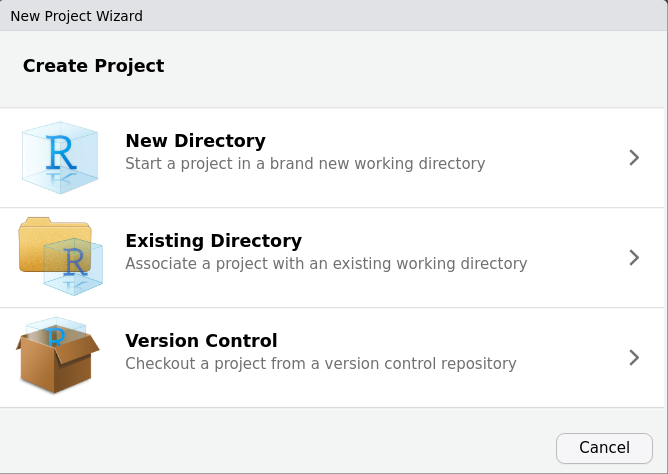
\includegraphics[width=4.40625in,height=\textheight]{images/create_project.png}

\begin{itemize}
\item
  This project was created in a new directory with a git repository
  setup alongside it

  \begin{itemize}
  \tightlist
  \item
    It is also advisable to open in a new session to clear your
    workspace and any loaded packages
  \end{itemize}
\end{itemize}

\hypertarget{section}{%
\subsubsection{\texorpdfstring{\protect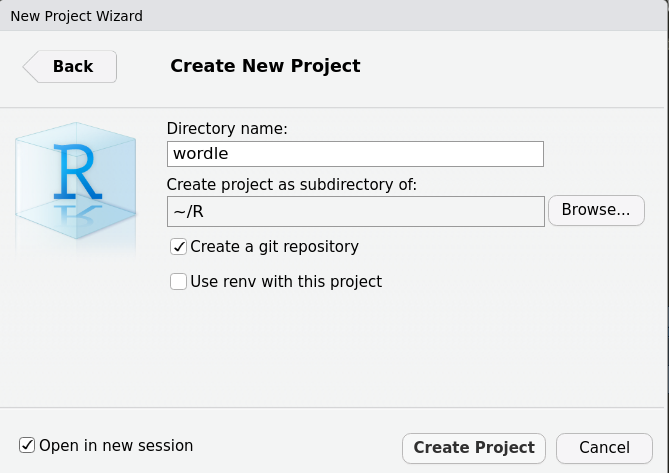
\includegraphics[width=4.41667in,height=\textheight]{images/project_settings.png}}{}}\label{section}}

\hypertarget{libraries}{%
\subsubsection{Libraries}\label{libraries}}

\begin{itemize}
\item
  \texttt{tidyverse} is \href{https://www.tidyverse.org/packages/}{a
  collection of packages} which greatly improve upon the basic
  functionality of R, and is usually worth loading at the start of every
  new project
\item
  \texttt{magrittr} is a handy \texttt{tidyverse} package, but is not
  loaded by default when
  \texttt{library(\textquotesingle{}tidyverse\textquotesingle{})} is
  called; it contains the very useful
  \texttt{\%\textless{}\textgreater{}\%} assignment pipe operator
\end{itemize}

\hypertarget{word-list}{%
\subsubsection{Word list}\label{word-list}}

\begin{Shaded}
\begin{Highlighting}[]
\FunctionTok{source}\NormalTok{(}\StringTok{\textquotesingle{}src/read\_data.R\textquotesingle{}}\NormalTok{)}

\FunctionTok{print}\NormalTok{(}\FunctionTok{head}\NormalTok{(words}\SpecialCharTok{$}\NormalTok{split))}
\end{Highlighting}
\end{Shaded}

\begin{verbatim}
##      [,1] [,2] [,3] [,4] [,5]
## [1,] "a"  "a"  "h"  "e"  "d" 
## [2,] "a"  "a"  "l"  "i"  "i" 
## [3,] "a"  "a"  "r"  "g"  "h" 
## [4,] "a"  "a"  "r"  "t"  "i" 
## [5,] "a"  "b"  "a"  "c"  "a" 
## [6,] "a"  "b"  "a"  "c"  "i"
\end{verbatim}

\begin{itemize}
\item
  We first load the raw Wordle word list from
  \texttt{data/word\_list.txt}
\item
  This list is then split into a character matrix for easier data
  handling

  \begin{itemize}
  \tightlist
  \item
    Don't hard-code values! If they release Wordle 2 next week using 6+
    letters instead of 5, this entire project should run without
    changing a single thing beyond the word list
  \end{itemize}
\end{itemize}

\hypertarget{letter-frequencies}{%
\subsection{Letter Frequencies}\label{letter-frequencies}}

\begin{itemize}
\item
  Expensive computations can be cached to speed up runtime next time
  \texttt{knitr::knit()} is called to generate a .pdf from the .rmd file
\item
  We can use \texttt{knitr::kable()} to neatly format R data structures
  into tables
\end{itemize}

\begin{Shaded}
\begin{Highlighting}[]
\FunctionTok{source}\NormalTok{(}\StringTok{\textquotesingle{}src/frequency\_tables.R\textquotesingle{}}\NormalTok{)}

\CommentTok{\# Create desired matrix}
\NormalTok{df }\OtherTok{=} \FunctionTok{do.call}\NormalTok{(cbind, }\FunctionTok{rev}\NormalTok{(frequencies))}

\CommentTok{\# Format to table and add column names}
\NormalTok{knitr}\SpecialCharTok{::}\FunctionTok{kable}\NormalTok{(df, }\AttributeTok{col.names =} \FunctionTok{c}\NormalTok{(}\FunctionTok{paste0}\NormalTok{(}\StringTok{\textquotesingle{}Position \textquotesingle{}}\NormalTok{, }\DecValTok{1}\SpecialCharTok{:}\NormalTok{n[}\DecValTok{2}\NormalTok{]), }\StringTok{\textquotesingle{}Total\textquotesingle{}}\NormalTok{))}
\end{Highlighting}
\end{Shaded}

\begin{longtable}[]{@{}lrrrrrr@{}}
\toprule
& Position 1 & Position 2 & Position 3 & Position 4 & Position 5 &
Total \\
\midrule
\endhead
a & 737 & 2263 & 1236 & 1074 & 680 & 5990 \\
b & 909 & 81 & 335 & 243 & 59 & 1627 \\
c & 922 & 176 & 392 & 411 & 127 & 2028 \\
d & 684 & 84 & 390 & 471 & 823 & 2452 \\
e & 303 & 1628 & 882 & 2327 & 1522 & 6662 \\
f & 598 & 24 & 178 & 233 & 82 & 1115 \\
g & 638 & 76 & 364 & 423 & 143 & 1644 \\
h & 489 & 546 & 120 & 235 & 370 & 1760 \\
i & 165 & 1383 & 1051 & 880 & 280 & 3759 \\
j & 202 & 11 & 46 & 29 & 3 & 291 \\
k & 376 & 95 & 272 & 503 & 259 & 1505 \\
l & 577 & 699 & 848 & 771 & 476 & 3371 \\
m & 693 & 188 & 511 & 402 & 182 & 1976 \\
n & 325 & 345 & 963 & 788 & 530 & 2951 \\
o & 262 & 2095 & 993 & 698 & 389 & 4437 \\
p & 859 & 231 & 364 & 418 & 147 & 2019 \\
q & 78 & 15 & 13 & 2 & 4 & 112 \\
r & 628 & 940 & 1198 & 719 & 673 & 4158 \\
s & 1565 & 93 & 533 & 516 & 3958 & 6665 \\
t & 815 & 239 & 616 & 898 & 726 & 3294 \\
u & 189 & 1187 & 667 & 400 & 67 & 2510 \\
v & 242 & 52 & 240 & 156 & 4 & 694 \\
w & 413 & 163 & 271 & 128 & 64 & 1039 \\
x & 16 & 57 & 133 & 12 & 70 & 288 \\
y & 181 & 271 & 213 & 108 & 1301 & 2074 \\
z & 105 & 29 & 142 & 126 & 32 & 434 \\
\bottomrule
\end{longtable}

\begin{Shaded}
\begin{Highlighting}[]
\CommentTok{\# Clean up}
\FunctionTok{rm}\NormalTok{(df)}
\end{Highlighting}
\end{Shaded}

\begin{figure}
\centering
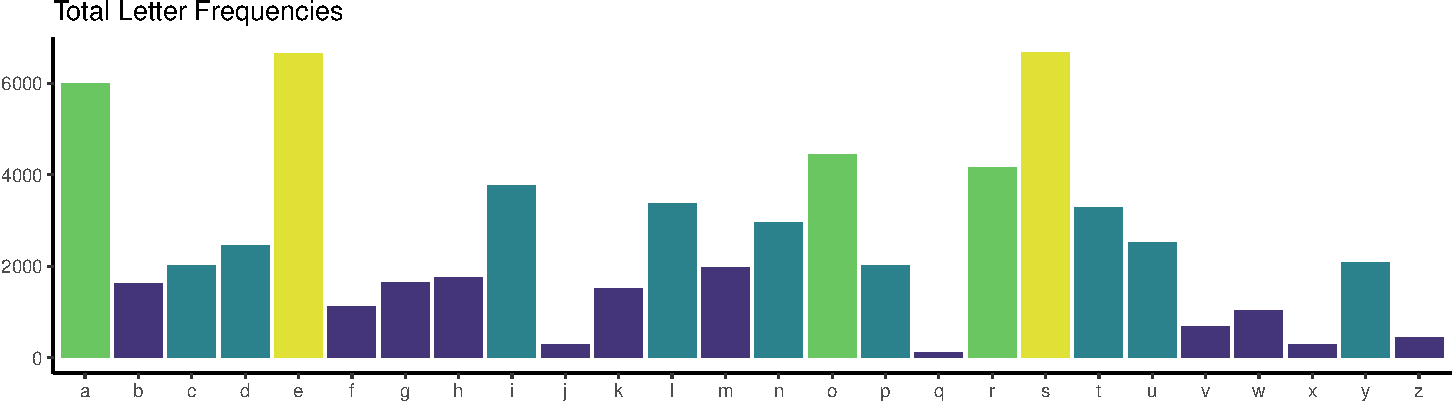
\includegraphics{report_files/figure-latex/letter-1.pdf}
\caption{\label{fig:fig-1}}
\end{figure}

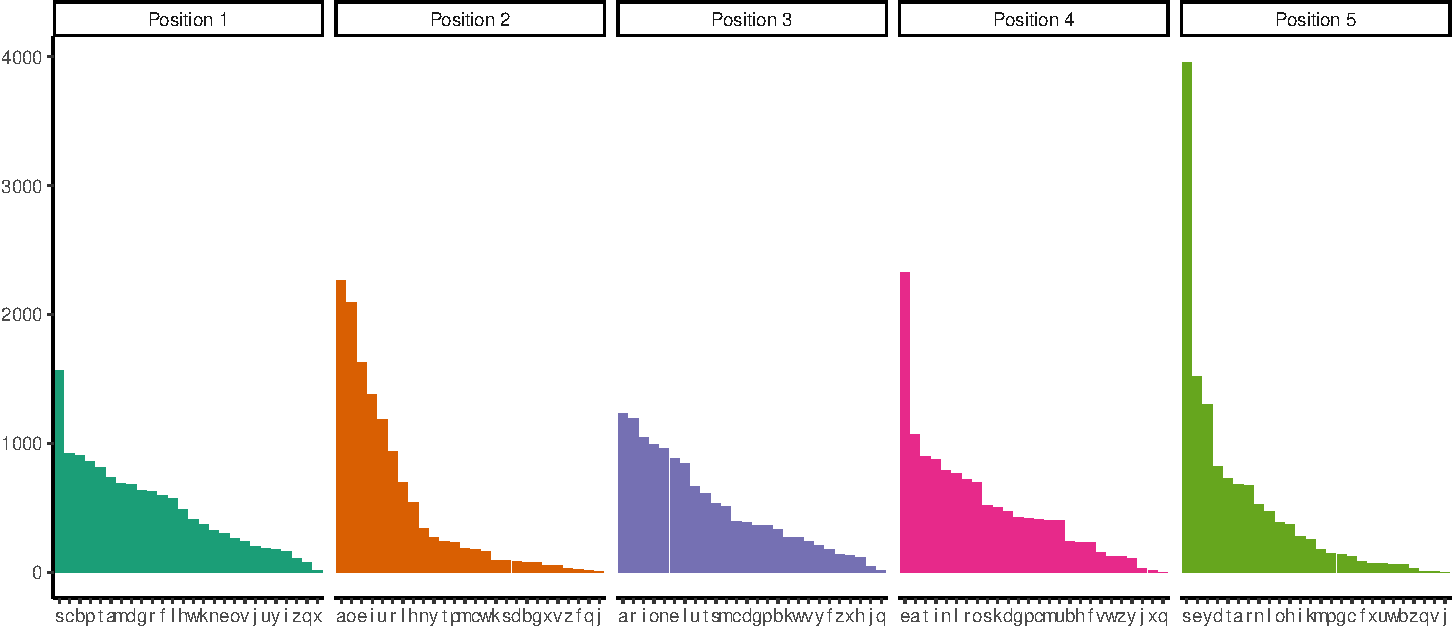
\includegraphics{report_files/figure-latex/positional-1.pdf}

\begin{itemize}
\item
  Here we have plots of the total and positional letter frequencies over
  the entire Wordle word list
\item
  Any changes in the script will be updated in the plot
\item
  Figure properties can be set in the chunk header e.g.,
  \texttt{\{r\ chunk-title,\ fig.height=3\}}
\item
  RMarkdown can create links to figure captions{[}\ref{fig:fig-1}{]} and
  \protect\hyperlink{initial-setup}{headings}
\end{itemize}

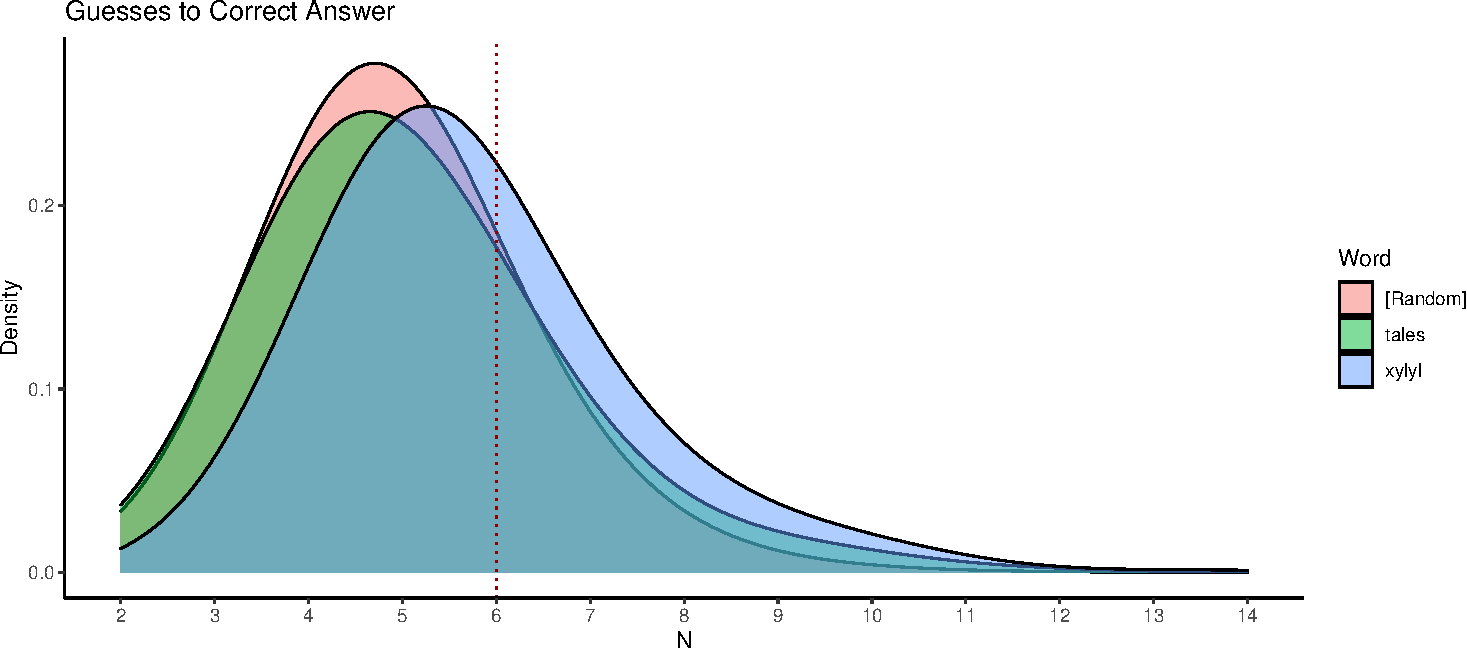
\includegraphics{report_files/figure-latex/bootstrapping-1.pdf}

\#TODO: Bootstrapping and data caches, simulated guess distribution
plots

\end{document}
